\section{Der Unterschied zwischen Javascript und Zero Code [FK]}
Die Entscheidung ob mit JavaScript Frameworks oder „Zero Code“ Frameworks gearbeitet werden soll muss bereits früh im Projekt geklärt werden weil es enorme Auswirkungen hat auf den Aufwand der eingeplant werden muss.
\section{JavaScript Frameworks}
JavaScript ist eine Skriptsprache und wurde erschaffen um CSS [\ref{sec:CSS}] und HTML [\ref{sec:HTML}] zu erweitern. Es kann verwendet werden, um Websites Interaktiver zu machen, sodass der/die BenutzerIn nicht jedes Mal eine vollständige neue Seite laden muss wenn er zum Beispiel eine neue Filteroption einer Liste auswählt. JavaScript kann aber noch viel mehr.
In unserem Fall könnte man JavaScript verwenden, um interaktive Grafiken auf einer Website zu platzieren. Dies hätte den Vorteil das der/die KundeIn das Diagramm nach seinen Wünschen anpassen könnte um die Daten anzuzeigen, welche er gerade benötigt. 
Nachteile bei der Verwendung von diversen JavaScript Frameworks sind zum Beispiel der große Aufwand, der von Nöten ist, weil man einen vollständigen Server mit Datenbankzugriff selber implementieren muss. Die Interaktivität muss man dabei ebenfalls selber integrieren. (vgl. \cite{JS})
Um einen besseren Überblick über die vorhandenen Libraries zu bekommen habe ich folgende untersucht: 
\subsection{D3}\label{ssec:D3}
\begin{figure}[H]
    
\includegraphics[scale=1]{images/d3logo.PNG}
    \caption{D3 (01.04.2020)}
    \centering
    \url{https://d3js.org/}
\end{figure}
„D3.js ist eine JavaScript-Bibliothek zur Manipulation von Dokumenten auf Basis von Daten. D3 hilft Ihnen, Daten mithilfe von HTML [\ref{sec:HTML}], SVG [\ref{sec:SVG}] und CSS [\ref{sec:CSS}] zum Leben zu erwecken. Die Betonung von D3 auf Webstandards gibt Ihnen die vollen Möglichkeiten moderner Browser, ohne sich an ein proprietäres Framework zu binden, und kombiniert leistungsstarke Visualisierungskomponenten mit einem datengesteuerten Ansatz zur DOM-Manipulation [\ref{sec:dom}].“~\cite{d3.js} 
\subsection{Google Charts}
Google Charts ist sehr ähnlich zu D3 [\ref{ssec:D3}] 
\section{Zero Code Frameworks}
Wie die Überschrift bereits vermuten lässt, handelt es sich bei „Zero Code“ Frameworks um Applikationen, die bereits vollständig implementiert worden sind. Der Arbeitsaufwand hält sich dementsprechend auch in gewissen Grenzen. Was aber nicht bedeutet, das gar keine Zeit investiert werden muss denn zusätzlich zu dem Installationsvorgang muss auch eine Datenbank- oder eventuell REST-Schnittstelle implementiert werden. Nachdem unser Arbeitgeber MIC die Vorgabe gab das wir mit einem „Zero Code“ Framework arbeiten sollen folgt nun eine detailliertere Form der getesteten Frameworks: (vgl. \cite{Anfang})
\subsection{Tableau}
\begin{figure}[H]
    
\includegraphics[scale=1]{images/tableauLogo.PNG}
    \caption{Tableau (01.04.2020)}
    \centering
    \url{https://de.wikipedia.org/wiki/Tableau_Software#/media/Datei:Tableau_Software_Logo_Small.png} 
\end{figure}
Tableau ist ein kostenpflichtiges Datenvisualisierungstool, das für große Daten in Unternehmen optimiert ist. Obwohl es eine überwältigende Menge an Möglichkeiten hat und dies einige Zeit zum Erlernen benötigt, ist es besonders für Nicht-Techniker sehr einfach, zu bedienen. Einmal richtig aufgesetzt können Datenfelder mithilfe von Drag n Drop einfach in das Diagramm gezogen werden und die Daten erscheinen im Diagramm. Es hilft auch bei der Auswahl der besten Grafik für jede Datenquelle, indem es Vorschläge anzeigt. Hat der/die BenutzerIn ein Diagramm fertig kann er es auch in die Cloud stellen damit alle berechtigten Nutzer darauf zugreifen können. (vgl. \cite{noauthor_tableau_2019-1})
\subsubsection{Vorteile}
\begin{itemize}
\item Einfaches einfügen der Daten durch Drag n Drop
\item Visualisierungen einfach über die Cloud teilen
\item Auf verschiedensten Geräten verwendbar
\end{itemize}
\subsubsection{Nachteile}
\begin{itemize}
\item Vergleichsweise Teuer
\item Nur als Desktop App verfügbar 
\item Schwierig zu Erlernen
\end{itemize}
\subsubsection{Tableau Preise}
Ein weiterer Wunsch von MIC war es, dass die verwendeten Technologien gratis sind oder nicht viel kosten. Tableau erreichte diese Anforderung eindeutig nicht, was die folgende Abbildung \ref{img:tableu_preise} über die Preispolitik zeigt. (vgl. \cite{noauthor_tableau_2019})
\begin{figure}[H]
    \centering
    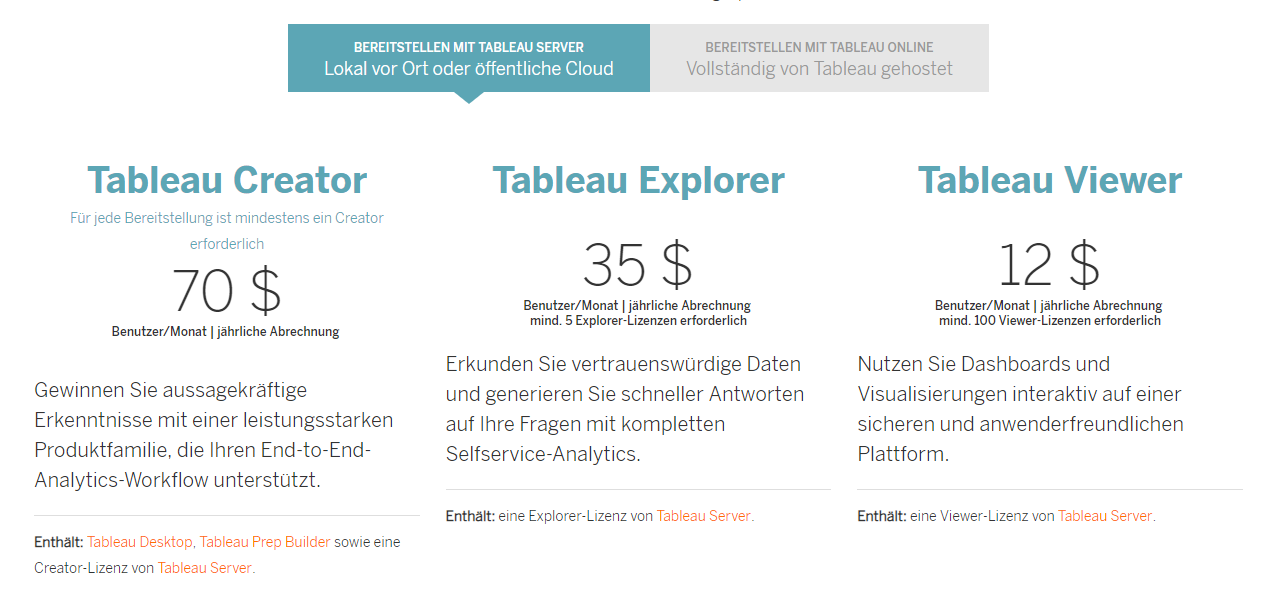
\includegraphics[scale=.45]{images/Tableau_Preise.png}
    \caption{Tableau Preispolitik (01.04.2020)}
    \url{https://www.tableau.com/de-de/pricing/teams-orgs}
    \label{img:tableu_preise}
\end{figure}
Zusätzlich kann man noch extra Pakete dazu bestellen
\subsection{Infogram}
\begin{figure}[H]
    
\includegraphics[scale=1]{images/infogramLogo.PNG}
    \caption{Infogram (01.04.2020)}
     \centering
     \url{https://static.crozdesk.com/web_app_library/providers/logos/000/000/214/original/infogram-1559230883-logo.png?1559230883} 
\end{figure}
Infogram ist ein Online-Werkzeug zur Erstellung von Grafiken und Diagrammen.
Es bietet 5 verschiedene Datenbanken (MySQL, Postgre, Amazon Redshift, Oracle und MS SQL Server), aber keine REST-Schnittstelle, da es hauptsächlich dazu dient, hübsche Grafiken für Präsentationen und Berichte zu erstellen.
Außerdem kann man Daten per Upload importieren, mit Google Drive, Drop Box und Json [\ref{sec:json}]. (vgl. \cite{noauthor_infogram_2019})
\subsubsection{Vorteile} 
\begin{itemize}
\item Sehr gut verwendbar für Presentationen
\item Einfach und Intuitiv zu benutzen
\item Online Teamarbeit an einem Document
\item Unglaublich schöne Grafiken
\end{itemize}
\subsubsection{Nachteile}
\begin{itemize}
\item Vergleichsweise Teuer
\item Keine Analysefunktionen
\item Nur eine kleine Auswahl an Funktionen und Grafiken
\item Keine REST-Schnittstelle
\end{itemize}
\subsubsection{Infogram Preise}
Infogram ist für seine Funktionen vergleichsweise teuer, ähnlich zu Tableau was in folgender Abbildung zu sehen ist \ref{img:infogram_preise} (vgl. \cite{noauthor_infogram_2019-1})
\begin{figure}[H]
    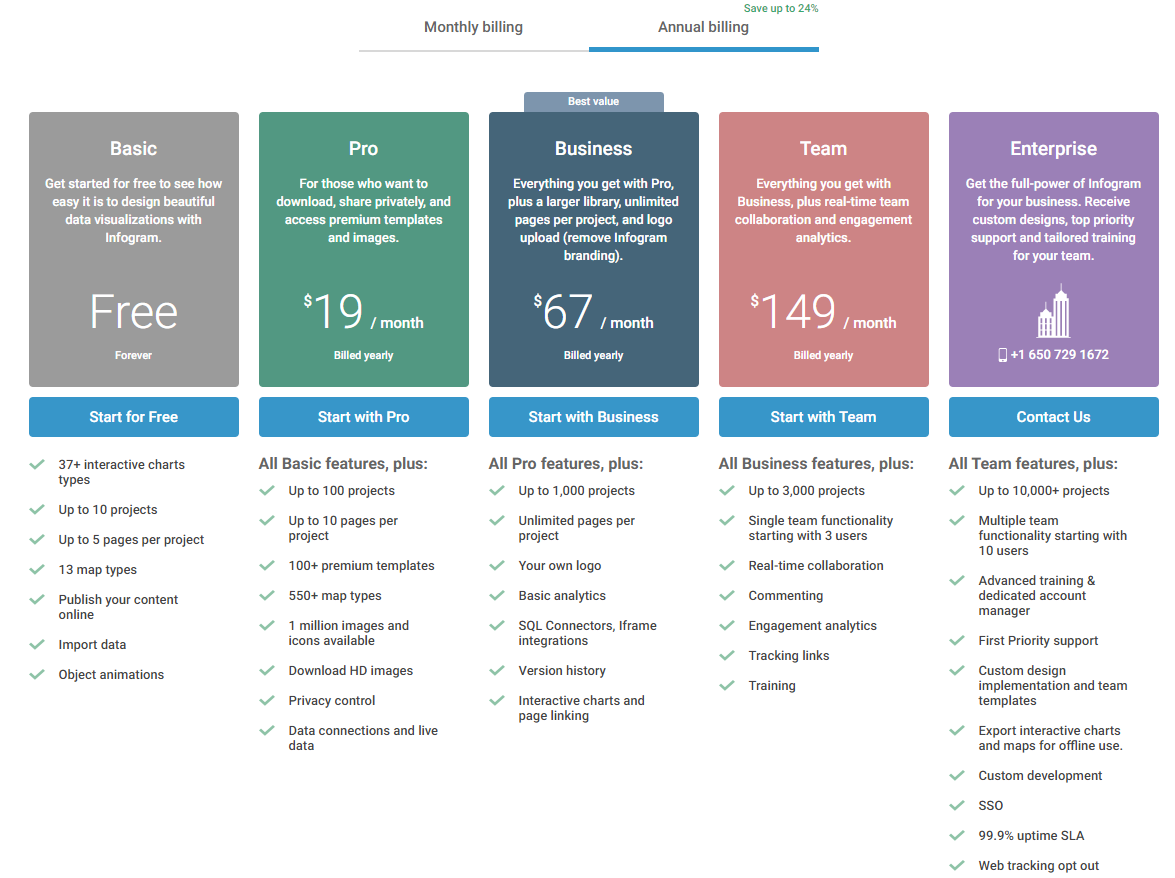
\includegraphics[scale=.50]{images/Infogram_Preise.png}
    \caption{Infogram Preispolitik (01.04.2020)}
    \url{https://infogram.com/pricing}
    \label{img:infogram_preise}
\end{figure}
\subsection{Chartblock}
\begin{figure}[H]
    
\includegraphics[scale=1]{images/chartblockLogo.PNG}
    \caption{Chartblock (01.04.2020)}
     \centering
     \url{https://assets-global.website-files.com/5a1eb87c9afe1000014a4c7d/5d78fa488f5b3e3a05a94567_Chartblocks%20logo.png} 
\end{figure}
Chartblock ist ein sehr einfaches Werkzeug, mit dem man Diagramme in einer Wizard-Form(Schritt-für-Schritt Anleitung) erstellen kann. Zur Zeit der Entscheidung, welches Tool verwendet werden soll, hatte es keine Möglichkeit Daten außer mit csv, Excel oder manuell zu importieren, daher ist es für unseren Anwendungsfall derzeit nicht relevant. (vgl. \cite{Chartblock})
\subsection{Datawrapper}
\begin{figure}[H]
    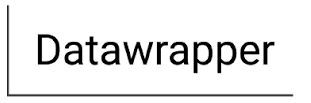
\includegraphics[scale=1]{images/dwLogo.PNG}
    \caption{Datawrapper (01.04.2020)}
     \centering
     \url{https://www.datawrapper.de/} 
\end{figure}
Datawrapper ist ähnlich zu Chartblock, jedoch liegt der Fokus auf Diagramme für Journalisten. Es hat ebenso keine Möglichkeit Daten aus einer Datenbank oder einer REST-Schnittstelle zu entnehmen weswegen es ebenfalls nicht infrage kommt.
\subsection{Qlik}
\begin{figure}[H]
    
\includegraphics[scale=1]{images/qlikLogo.PNG}
    \caption{Qlik (01.04.2020)}
     \centering
     \url{https://bdg.io/wp-content/uploads/qlik_logo_neu.jpg} 
\end{figure}
Qlik ist ein Tool mit Schwerpunkt Data Analytics. Es kann aber auch Diagramme zeichnen.
Qlik kann Daten aus allen gängigen Quellen verarbeiten und es schlägt dabei auch vor, wie Datensätze verbunden werden könnten was einiges an Aufwand spart. Auch bei der gemeinsamen Erstellung und Verteilung von Daten hilft Qlik. Sodass auch Nicht-Techniker die Informationen Nützen und verwenden können. (vgl. \cite{qlik_using_2017}, \cite{noauthor_swapi_2019}, \cite{noauthor_qlik_nodate}, \cite{noauthor_qlik_2019-1}, \cite{noauthor_qlik_2019-2},\cite{noauthor_qlik_2019-3})
\subsubsection{Vorteile} 
\begin{itemize}
\item Code freie Daten Analysefunktionen mit Künstlicher Intelligenz
\item Auf allen gängigen Plattformen benutzbar
\item Legt großen Wert auf Zusammenarbeit
\item Viele Datenimport Möglichkeiten darunter REST
\item Hohe Skalierbarkeit mit Multi-Nodes
\item Interaktive Diagramme
\end{itemize}
\subsubsection{Nachteile}
\begin{itemize}
\item Der Preis ist nicht ersichtlich, weil er für jeden Kunden einzeln berechnet wird
\item Es gibt Programme die deutlich schönere Grafiken und Diagramme erzeugen
\end{itemize}

\subsection{Power Bi}
\begin{figure}[H]
    
\includegraphics[scale=0.6]{images/PowerBiLogo.PNG}
    \caption{Power Bi (01.04.2020)}
     \centering
     \url{https://o365reports.com/wp-content/uploads/2016/10/PowerBI-e1557666264791.jpg} 
\end{figure}
PowerBI ist das Business-Intelligence-Tool von Microsoft. Es ist einfach, zu bedienen und hat sehr schöne Diagramme out-of-the-box. Leider konnte ich die REST-API nicht ausprobieren, weil man das online registrieren muss und Admin-Berechtigungen von MIC benötigt. Es gibt aber Testdaten mit denen man zumindest den Diagrammteil der Applikation ausprobieren kann. Die Benutzung ist sehr einfach auch ohne technische Erfahrung und die Diagramme sind wirklich sehr schön. (vgl. \cite{noauthor_power_2019-1},\cite{noauthor_downloads_2019},\cite{rkarlin_what_2019},\cite{noauthor_power_2019})
\begin{itemize}
\item Interaktive Diagramme
\item Sehr Intuitiv in der Benutzung auch ohne Technische Erfahrung
\item Sehr schöne Diagramme
\item Es können Datenabfragen mit Volltextsuche gemacht werden (nur auf Englisch)
\item Eigene Analysefunktionen geschrieben in Python oder R
\item Auf allen gängigen Plattformen benutzbar
\end{itemize}
\subsubsection{Nachteile}
\begin{itemize}
\item Der Preis ist nicht ersichtlich, weil er für jeden Kunden und jede Kundin einzeln berechnet wird
\item Es gibt Programme die deutlich schönere Grafiken und Diagramme erzeugen
\end{itemize}
Die Tatsache das Power Bi fast ausschließlich in der Cloud läuft, kann sowohl Vorteile als auch Nachteile bieten. Ein klarer Vorteil dabei wäre das sich MIC nicht eigene Server bauen oder vorhandene Server belasten müsste. Ein Nachteil wäre die starke Abhängigkeit von dem Cloud.
\subsubsection{Power Bi Preispolitik}
Microsoft verlangt für seinen Enterpriseservice nicht Pro Benutzer, sondern Pro benutzter Rechen- und Speicherkapazität. Wie in folgender Abbildung ersichtlich wird, gibt es aber auch ein Pro Benutzer Abonnement: (vgl. \cite{noauthor_powerbi_2019})
\begin{figure}[H]
    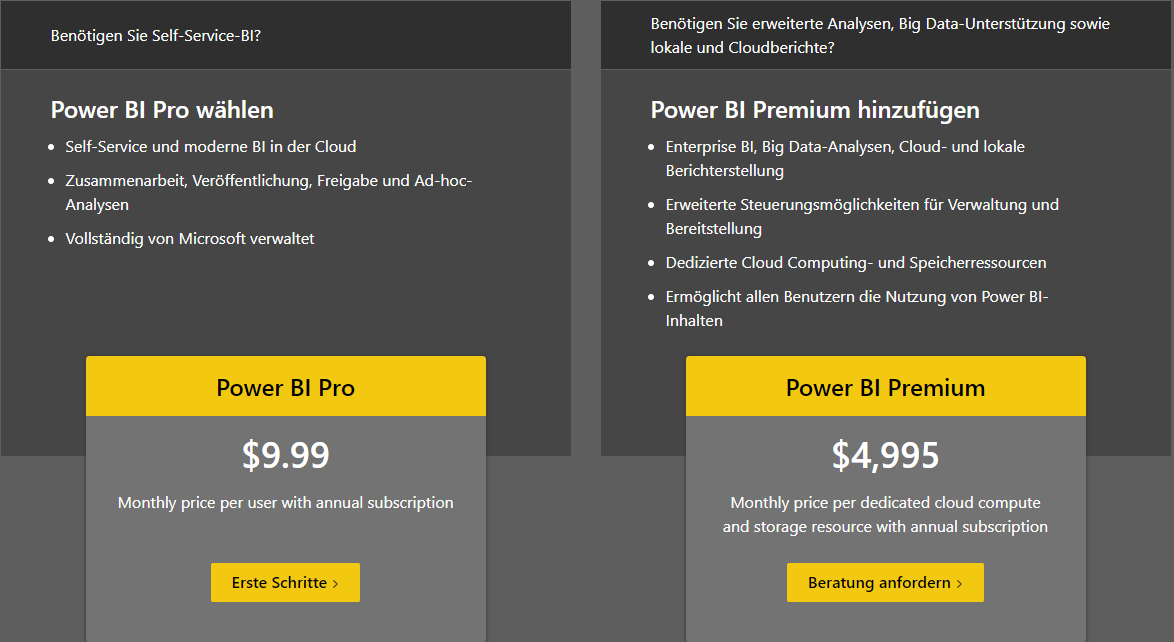
\includegraphics[scale=.60]{images/PowerBi_Preise.png}
    \caption{PowerBI Preispolitik (01.04.2020)}
    \url{https://powerbi.microsoft.com/de-de/pricing/}
    \label{img:powerbi_preise}
\end{figure}

\subsection{Kibana}\label{ssec:Kibana}
\begin{figure}[H]
    
\includegraphics[scale=0.6]{images/kibanaLogo.PNG}
    \caption{Kibana (01.04.2020)}
     \centering
     \url{https://lh3.googleusercontent.com/proxy/L4FRW5tQ05yEJhUf4qHfIx_ch0IYysxhiLztinrsy811Ub2D0JIaRWy_sZ01w-8CnbXPWw-lbnlQCQrPkZQVJHPJCfaSDG7lBZ1QvB0sx6rauKTQJnB7goICYsZQ} 
\end{figure}
Kibana ist ein grafisches Werkzeug, das auf Elasticsearch basiert. Elasticsearch ist eine dokumentbasierte NoSQL Datenbank, welche durch Features wie Volltextsuche und extrem schnelle Suchabfragen glänzt. Eine weitere tolle Eigenheit ist das Kibana sowohl als auch Elasticsearch schnell über Docker aufgesetzt werden können und sofort Startbereit sind und Daten über REST-Schnittstelle oder Zugriff auf externe Datenbanken importiert werden können. Kibana bietet aber auch out-of-the-box die Möglichkeit, Musterdatensätze zu verwenden um einen ersten Eindruck zu erhalten. Kibana dient nicht nur zur Visualisierung, sondern auch zur Überwachung von Abfragen auf Daten. So kann z.B. kontrolliert werden, von wem die Daten benutzt werden. (vgl. \cite{noauthor_kibana_2015},\cite{noauthor_kibana:_2019},\cite{noauthor_indices_2019})
\begin{itemize}
\item Umfassendes Berechtigungssystem
\item Sehr einfach aufzusetzen
\item Schöne Diagramme
\item Es können Datenabfragen mit Volltextsuche gemacht werden (nur auf Englisch)
\item Sehr schnell durch die Elasticsearch Suchmaschine
\item REST-Schnittstelle verfügbar
\item Hochgradig Interaktive Diagramme
\item Sehr gute Skalierbarkeit dank Multi-Nodes
\item Opensource und Großteils Gratis
\end{itemize}
\subsubsection{Nachteile}
\begin{itemize}
\item Erweiterte Sicherheitsfunktionen, Multi-Nodes [\ref{sec:Node}], Machine Learning und Support kosten etwas
\item Diagramme erstellen dauert etwas ist etwas komplexer als bei anderen Visualisierungs Programmen
\end{itemize}
\section{Andere Tools}
\subsection{Dash by Plotly}
\begin{figure}[H]
    
\includegraphics[scale=1.3]{images/plotlyLogo.PNG}
    \caption{Dash (01.04.2020)}
    \centering
    \url{https://plotly.com/} 
\end{figure}
Dash ist eine Open-Source-Bibliothek für R und Python. Es wird kein JavaScript benötigt, aber Python. Mit Python schreibt man sowohl das Layout der Website sowohl als auch die Logik des Servers dahinter. Somit erreicht es einen ähnlich großen Funktionsumfang wie oben genannte JavaScript Frameworks mit dem bedeutenden Unterschied das Python mit wenigen Zeilen Code sehr viel mehr bewirken kann als JavaScript. Jedoch muss hier jedes Diagramm und Dashboard von einem Programmierer entwickelt werden. Einfache Kunden können somit nur schwer Änderungen an dem Diagramm vornehmen oder gar neue erstellen. (vgl. \cite{noauthor_dash_2019}, \cite{noauthor_dash_2019-1})
\subsubsection{Vorteile} 
\begin{itemize}
\item Gratis Benutzung der Bibliotheken. Nur der Support ist kostenpflichtig
\item Kann gut in Webseiten eingebunden werden
\item REST-Schnittstelle kann selber geschrieben werden
\item Die Interaktivität der Diagramme wird von den Dash Bibliotheken unterstützt => Weniger Aufwand bei der Implementierung
\end{itemize}
\subsubsection{Nachteile}
\begin{itemize}
\item Implementierungen notwendig
\item Analysefunktionen müssen selber geschrieben werden
\item Nicht-Techniker können keine eigenen Diagramme erstellen
\end{itemize}
\section{Vergleich der Visualisierungs Applikationen}
Es gibt noch viel mehr Visualisierungsprogramme aber die wohl wichtigsten / bekanntesten sind hier gelistet. Eine paar der oben gelisteten Programme sind Nischenprodukte, es wird bestimmte Einsatzzwecke für Applikationen wie z.B. Chartblock geben jedoch werden diese nicht für die folgende Top 3 reichen. 
Zur Erinnerung hier die Anforderungen von MIC für ein Visualisierungs Tool.
\subsection{Dritter Platz: Qlik}
Qlik ist nicht schlecht, aber im Vergleich zu Kibana und PowerBI ist das Einrichten von Beziehungen und das Erstellen von Diagrammen etwas komplexer. Wenn man z.B. Daten von einer REST-Verbindung erhält, erzeugt es einige Spalten mehr als im Original-Datensatz, was sehr irritierend ist und für einen erhöhten Aufwand in der REST-Schnittstellenimplementierung sorgt. Ein weiterer wichtiger Punkt ist, dass Qlik-Benutzer sich über den hohen RAM-Bedarf beschweren welcher bei der geplanten Hochskalierung der Hardwareressourcen zu bedeutenden Kostenerhöhungen führen wird. Somit fällt Qlik trotz der guten analytischen Funktionen auf Platz 3.
\subsection{Zweiter Platz: Power Bi}
Die Entscheidung zwischen PowerBI und Kibana war eine schwere Wahl, weil PowerBI wirklich schön und einfach zu bedienen ist. Darüber hinaus hat es einige Features wie die "Voll Text Abfragen" und "On-Click-Analyse", die sie sehr gut machen. Leider konnte ich die REST-API aufgrund eines komplexen Azure (Cloud von Microsoft) Registrierungsmechanismus nicht überprüfen. Ein entscheidender Faktor war die Auslieferung (Deployment) von PowerBI. Es gibt nur ein zusätzliches Tool namens "PowerBI Report Server", das nur dazu dient, Berichte innerhalb einer Firma zu verbreiten, die vorher in PowerBI Desktop gemacht wurden. Dieses eine Programm läuft auf einem Server in der Firma, die es einsetzt. Der ganze Rest Verarbeitung der Visualisierung und der analytischen Funktionen übernimmt die Microsoft Cloud Azure. Dadurch wird das Produkt nicht nur deutlich teurer, sondern die Firma wird auch sehr viel stärker an Microsoft gebunden.
\subsection{Erster Platz: Kibana}
Kibana ist gleich in den meisten Punkten mit PowerBI, aber es gibt zwei wichtige Punkte, die Kibana ein wenig besser machen:
\begin{enumerate}
\item Kibana und Elasticsearch sind out-of-the-box für den Einsatz auf Servern konzipiert, was die Bereitstellung und den Zugriff von vielen verschiedenen Geräten aus erleichtert, ohne dass eine Desktop-Applikation installiert werden muss.
\item Besonders Elasticsearch ist (wie beworben) sehr schnell, da es für den Anwendungsfall gebaut ist für Analysefunktionen niedrige Zugriffszeiten zu bieten.
\end{enumerate}